\section{Vecinos más cercanos}

% \todo[inline]{Como esta representada nuestra informacion}
% Todas las imágenes de nuestro set de datos tiene una dimensión de 28x28 píxeles (En total 784 píxeles). Al cargar una imagen, la guardaremos como un vector de 784 coordenadas. Y BLAH

Nuestro problema consiste en tomar una imagen de un dígito manuscrito, y decidir cuál es el dígito que representa. Escrituras de un mismo dígito para distintas personas pueden ser muy diferentes entre sí, e incluso en ocasiones puede ser complicado para un ser humano distinguirlos. \\

{\centering
    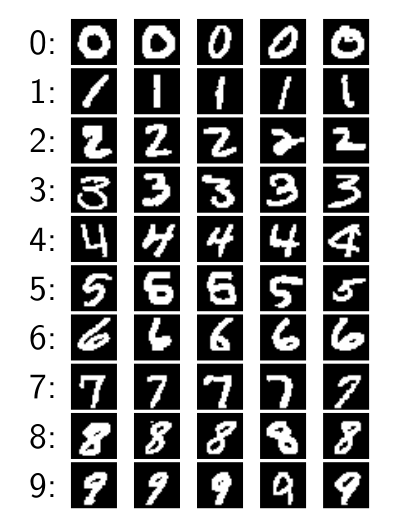
\includegraphics[scale=0.40]{informe/imagenes/knn/muestraVariaciones.png} \\
    \captionof{figure}{Algunas muestras diferentes para los mismos dígitos. \\
    (Fuente de imagen: Clase de laboratorio) \\ }
}
$ $\newline

El primer método que presentaremos para resolver este problema, es el método de \textit{k-Vecinos más cercanos}, o en inglés \textit{k-Nearest Neighbors}. De ahora en más utilizaremos indistintamente el nombre \textbf{kNN} por sus sigles en inglés. \\

Tenemos diez categorias posibles (los dígitos 0-9) y un conjunto de imágenes para las cuáles conocemos el dígito que representan. Llamaremos a este conjunto de imágenes el \textit{conjunto de datos etiquetados}. Dado un nuevo dato \textbf{sin etiquetar}, queremos decidir a qué categoría pertenece. La forma más natural para clasificarlo, es compararlo con nuestros datos conocidos y elegir la categoría a la cuál más se \textit{parezca}. \textit{kNN} es una implementación y una generalización de esta idea. \\


\todo[inline]{Por que nos sirve en nuestro problema? como lo usamos?}

\todo[inline]{Usar alguna imagen ilustrativa}

\todo[inline]{Implementacion, quiza hablar sobre optimizaciones y estructuras, minheap y eso}

\todo[inline]{Cuales son los posibles problemas que traeria? Dimensionalidad. Aclarar que corroboraremos esto en la seccion de experimentacion}


\section{PSA}

\todo[inline]{Que es psa}

\todo[inline]{Por que usariamos psa en nuestro problema}

\todo[inline]{Explicar con detalle el metodo}

\todo[inline]{Mencionar que necesitamos los autovec pero explicar como en la seccion siguiente}

\todo[inline]{Posibles problemas? Muy costoso crear la matriz de covarianza si tenemos una muestra muy grande}



\section{Método de la potencia y Deflación}

Cómo habíamos mencionado, para poder diagonalizar la matriz de covarianza necesitamos conseguir los autovalores y autovectores. Conseguir los autovalores de la manera tradicional implica encontrar las raíces de un polinomio de grado 784, y no es algo que estemos dispuestos a intentar. Utilizaremos entonces el método iterativo conocido como \textit{Método de la potencia}.
\begin{algorithm}
    \caption{Método de la potencia (Matriz $B$, Vector $x_0$, Int $iters$)}
    \begin{algorithmic}[h]
        \State{$v \gets x_0$}
        \For{$i \gets 1$ to $iters$}
            \State{$v \gets \frac{Bv}{\norm{Bv}}$} \\
        \EndFor
        \State  $\lambda \gets \frac{v^tBv}{v^tv}$
        \State return $(\lambda, v)$

    \end{algorithmic}
\end{algorithm}

Podemos estar seguros de que los autovalores son números reales positivos, pues la matriz de covarianza es una matriz simétrica. Además, también por ser simétrica sabemos que vamos a poder conseguir una base de autovectores ortonormales, que es exactamente lo que necesitamos. \\

Con el método de la potencia conseguimos únicamente el autovalor dominante (y un autovector correspondiente). Como queremos conseguir una base, extendemos el método de la potencia utilizando el método de deflación. Esto funciona por la siguiente observación:

$$ B - \lambda v_1 {v_1}^{t} \text{\hspace{1cm}tiene los mismos autovalores que B (excepto $\lambda$).} $$

Por lo tanto, cuando apliquemos el método de la potencia en la matriz resultante, el autovalor que conseguiremos será distinto del $\lambda$ obtenido inicialmente. \\

Otro detalle es que el vector inicial $x_0$ es elegido aleatoriamente. Si bien es posible en teoría que con un cierto $x_0$ el método no converja, en la práctica eso no sucede. En primer lugar, hay muy pocas probabilidades de tomarlo, y en segundo lugar, los errores de precisión juegan a nuestro favor, ya que con una mínima desviación el $x_0$ deja de ser problemático. \\

El último factor a tener en cuenta es la cantidad de iteraciones para la convergencia. Para que pasen los tests de la cátedra es necesario hacer más de 1000 iteraciones. Sin embargo, como veremos en la sección de experimentación, con una cantidad muchísimo menor de iteraciones el accuaracy obtenido no se modifica, por lo que tomaremos una cantidad mucho menor de iteraciones para optimizar el tiempo de ejecución. \\

\section{K-Fold Cross Validation}

A lo largo de la experimentación, entrenaremos nuestro sistema con un cierto conjunto de datos y luego clasificaremos muestras. Como queremos saber qué tan bien o qué tan mal funciona nuestra sistema, estas muestras estarán etiquetadas para poder comparar el grupo real con el grupo predicho. \\

Dado que nuestra base de información es, si bien extensa, limitada, surge la pregunta de cómo elegir cuáles datos entrenar y cuáles clasificar. Más aún, si tomamos siempre los mismos datos, los mejores parámetros que obtengamos serán para ese set de datos en particular, y esto no es algo deseable (el problema mencionado es conocido como \textit{overfitting}). Para resolver estas problemáticas, utilizaremos la técnica de \textit{K-Fold Cross Validation}. \\

El método consiste en particionar nuestro espacio de muestras en $K$ grupos (a partir de ahora, \textit{folds}) y utilizar $K - 1$ folds como datos de entrenamiendo y el fold restante para testeo. Fijados $K$ y los demás parámetros necesarios para nuestro entrenamiento, ejecutaremos el método $K$ veces, donde en cada iteración se varía cuál es el fold que se utilizará para testear. Al finalizar cada iteración se obtendrá un valor correspondiente a cierta métrica (por ejemplo $accuaracy$) y el resultado final será el promedio de todas las iteraciones. \\

{\centering
    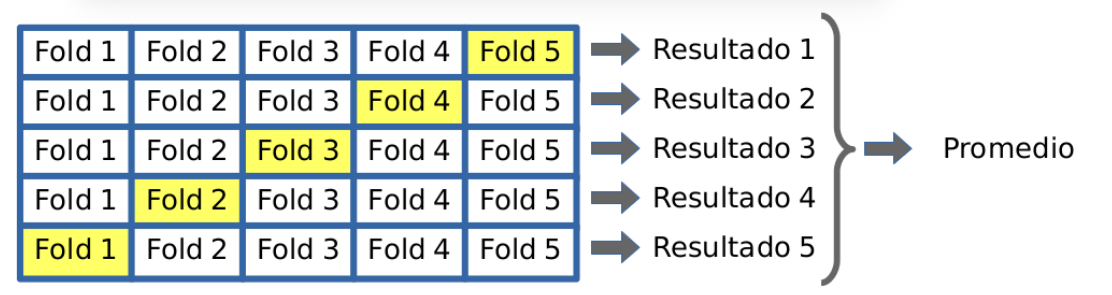
\includegraphics[scale=0.30]{informe/imagenes/kfold/kfoldEjemplo2.png} \\
    \captionof{figure}{Ejemplo de K-fold con K = 5. \\
    (Fuente de imagen: Clase de laboratorio) \\ }
}
$ $\newline
Dado que nuestra clasificación no es binaria, los datos que obtendremos serán para cada una de las 10 categorías, y la efectividad de los parámetros se analizará por separado. Es posible que nuestro clasificador sea muy bueno para ciertos dígitos pero que sea malo para otros. \\

\todo[inline]{No se si vale la pena mencionar la implementacion, pensar que mas}


